\section{Results And Testing} \label{sec:results_and_testing}
During the automated training and selection process, the SVM classifier is selected as the best-suited model for dataset 1, dataset 2, and dataset 4. Whereas RF classifier is selected as the best-suited model for dataset 3. 

Performance metrics used for evaluation were Accuracy, F1, Precision, Recall, Area under ROC Curve, and Total prediction time. The weightage assigned to these metrics for ranking was 0.65, 0.5, 0.6, 0.6, 0.5, 3 respectively. Where lower value means higher priority.

\subsection{Performance Evaluation} \label{subsec:performance_evaluation}
The models are tested with a testing dataset obtained from MIT-BIH database. Testing dataset consists of 5473 signals. Figure \ref{fig:perfromance_results_dataset_1}, \ref{fig:perfromance_results_dataset_2}, \ref{fig:perfromance_results_dataset_3} and \ref{fig:perfromance_results_dataset_4} shows that model trained with automated system produced satisfactory results. Few models like KNN, RF, and SVM performed better than other models (DT) at the cost of higher prediction time. Whereas MLP models produced good overall results with lower prediction time.

% Best model Performance tabular
\begin{table}[hbt]
\caption{Performance of models trained on dataset 1} \label{tab:performance_of_models_trained_on_dataset_1}
\begin{tabular*}{\tblwidth}{@{}LLLLLL@{}}
    \toprule
    Metric & KNN & DT & MLP & RF & \textbf{SVM} \\
    \midrule
    Accuracy & 96.72 & 94.46 & 96.89 & 97.33 & \textbf{97.40} \\
    F1 & 89.71 & 83.43 & 90.05 & 91.30 & \textbf{91.69} \\
    Precision & 92.53 & 81.86 & 94.71 & 97.95 & \textbf{96.43} \\
    Recall & 87.06 & 85.06 & 85.84 & 85.50 & \textbf{87.40} \\
    ROC & 92.84 & 90.68 & 92.45 & 92.57 & \textbf{93.38} \\
    Time(s) & 0.457 & 0.001 & 0.002 & 0.015 & \textbf{0.297} \\
    \bottomrule
\end{tabular*}
\end{table}

\begin{table}[hbt]
\caption{Performance of models trained on dataset 2} \label{tab:performance_of_models_trained_on_dataset_2}
\begin{tabular*}{\tblwidth}{@{}LLLLLL@{}}
    \toprule
    Metric & KNN & DT & MLP & RF & \textbf{SVM} \\
    \midrule
    Accuracy & 96.83 & 95.04 & 96.69 & 97.09 & \textbf{97.46} \\
    F1 & 90.28 & 85.50 & 89.73 & 90.75 & \textbf{92.15} \\
    Precision & 94.25 & 84.90 & 94.73 & 98.60 & \textbf{96.79} \\
    Recall & 86.63 & 86.09 & 85.23 & 84.05 & \textbf{87.93} \\
    ROC & 92.77 & 91.48 & 92.13 & 91.90 & \textbf{93.66} \\
    Time(s) & 0.435 & 0.001 & 0.003 & 0.014 & \textbf{0.295} \\
    \bottomrule
\end{tabular*}
\end{table}

\begin{table}[hbt]
\caption{Performance of models trained on dataset 3} \label{tab:performance_of_models_trained_on_dataset_3}
\begin{tabular*}{\tblwidth}{@{}LLLLLL@{}}
    \toprule
    Metric & KNN & DT & MLP & \textbf{RF} & SVM \\
    \midrule
    Accuracy & 97.07 & 94.64 & 96.41 & \textbf{97.22} & 97.44 \\
    F1 & 90.93 & 84.30 & 89.34 & \textbf{91.21} & 92.00 \\
    Precision & 95.82 & 83.81 & 90.13 & \textbf{98.37} & 97.81 \\
    Recall & 86.53 & 84.80 & 88.57 & \textbf{85.02} & 86.85 \\
    ROC & 92.87 & 90.73 & 93.29 & \textbf{92.36} & 93.22 \\
    Time(s) & 0.404 & 0.001 & 0.002 & \textbf{0.017} & 0.293 \\
    \bottomrule
\end{tabular*}
\end{table}

\begin{table}[hbt]
\caption{Performance of models trained on dataset 4} \label{tab:performance_of_models_trained_on_dataset_4}
\begin{tabular*}{\tblwidth}{@{}LLLLLL@{}}
    \toprule
    Metric & KNN & DT & MLP & RF & \textbf{SVM} \\
    \midrule
    Accuracy & 96.84 & 94.99 & 95.34 & 96.88 & \textbf{97.15} \\
    F1 & 90.52 & 85.73 & 85.01 & 90.37 & \textbf{91.39} \\
    Precision & 95.71 & 85.91 & 97.83 & 98.65 & \textbf{97.41} \\
    Recall & 85.86 & 85.55 & 75.15 & 83.37 & \textbf{86.07} \\
    ROC & 92.52 & 91.28 & 87.40 & 91.56 & \textbf{92.79} \\
    Time(s) & 0.452 & 0.001 & 0.002 & 0.014 & \textbf{0.294} \\
    \bottomrule
\end{tabular*}
\end{table}

% Best model Performance chart
\begin{figure}[btp]
    \centering
    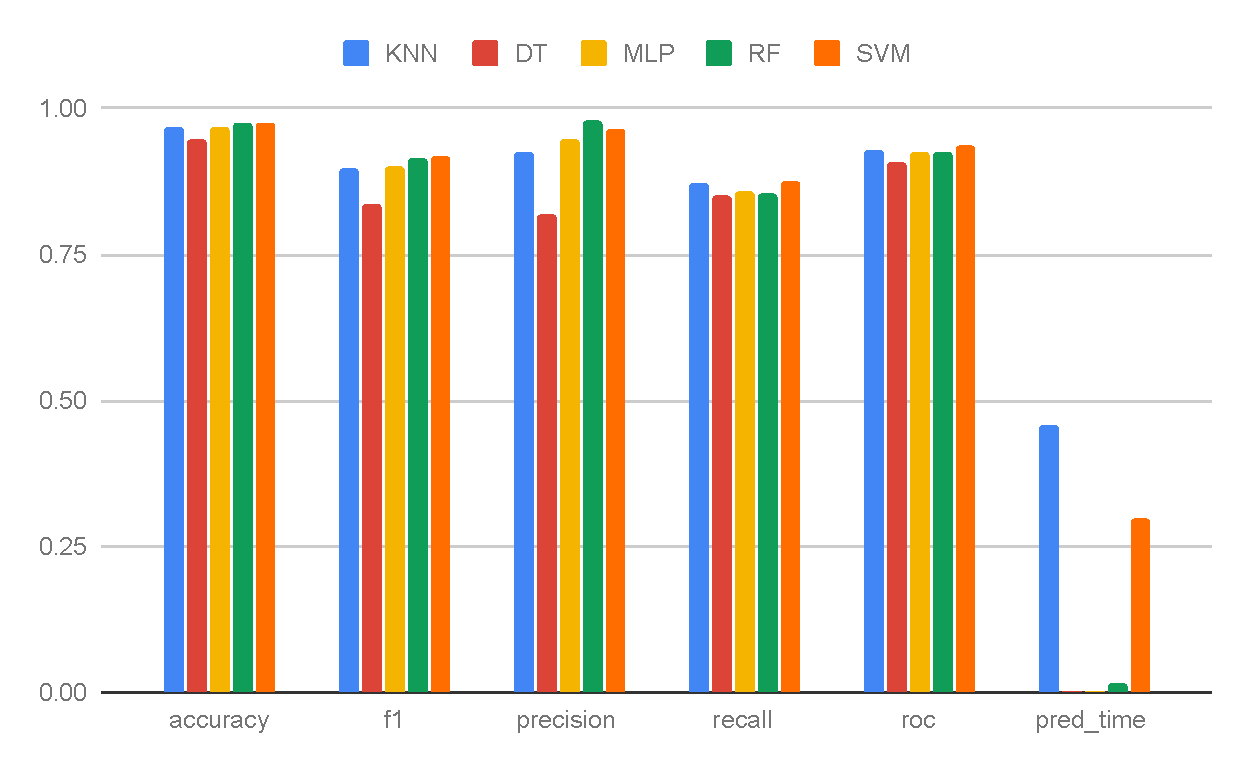
\includegraphics[width=0.9\columnwidth]{media/results/perf_ds_1.pdf}
    \caption{Performance Results Dataset 1} \label{fig:perfromance_results_dataset_1}
\end{figure}

\begin{figure}[btp]
    \centering
    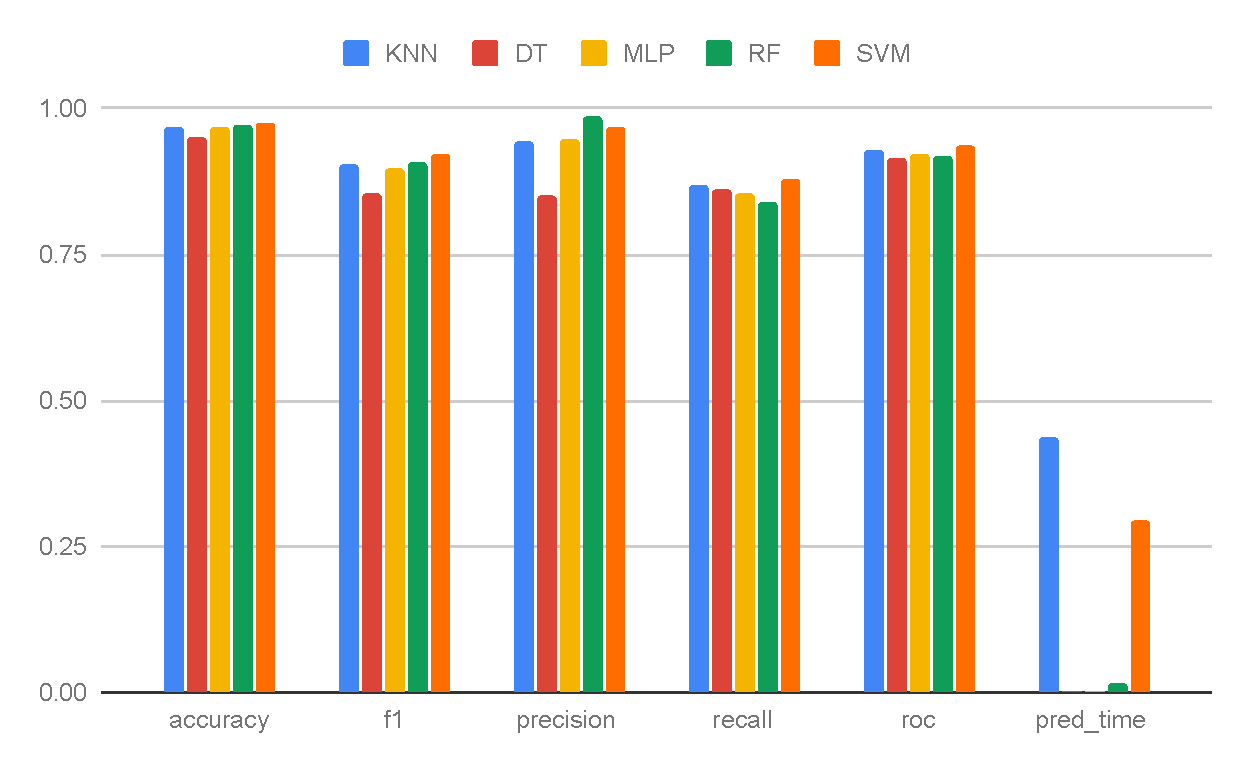
\includegraphics[width=0.9\columnwidth]{media/results/perf_ds_2.pdf}
    \caption{Performance Results Dataset 2} \label{fig:perfromance_results_dataset_2}
\end{figure}

\begin{figure}[btp]
    \centering
    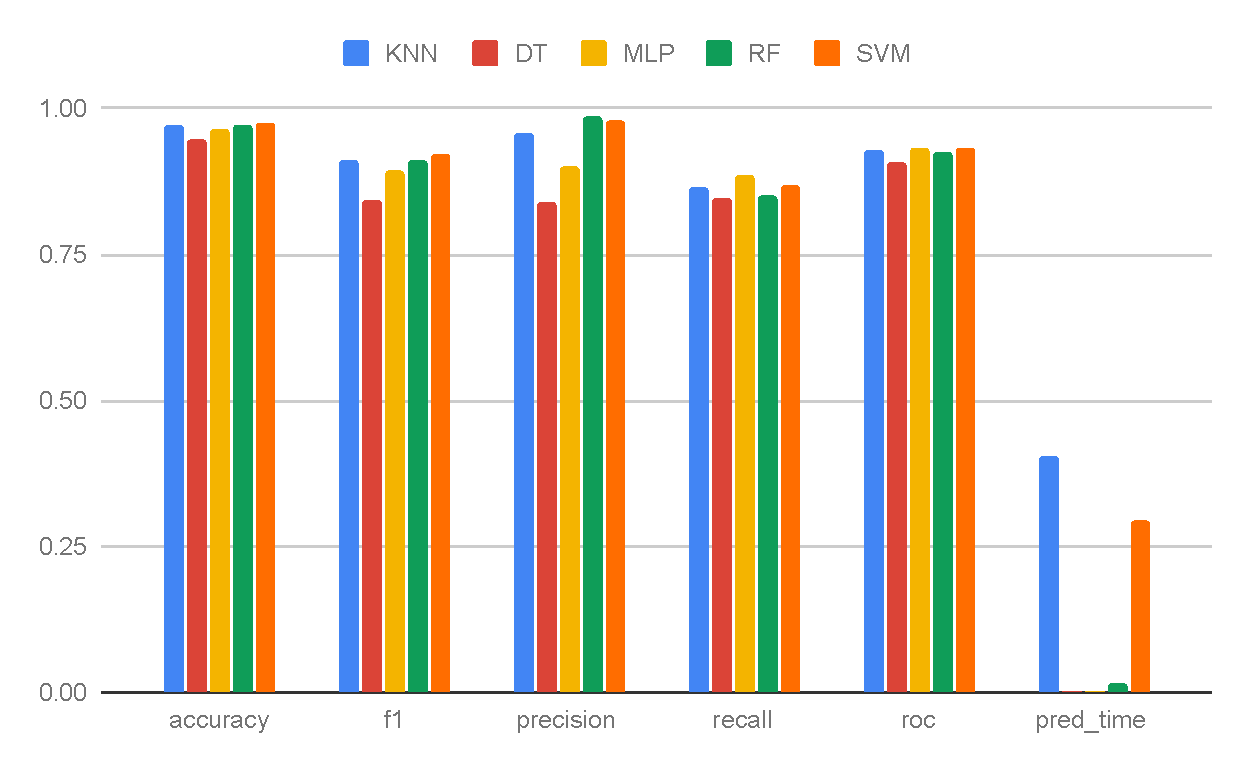
\includegraphics[width=0.9\columnwidth]{media/results/perf_ds_3.pdf}
    \caption{Performance Results Dataset 3} \label{fig:perfromance_results_dataset_3}
\end{figure}

\begin{figure}[btp]
    \centering
    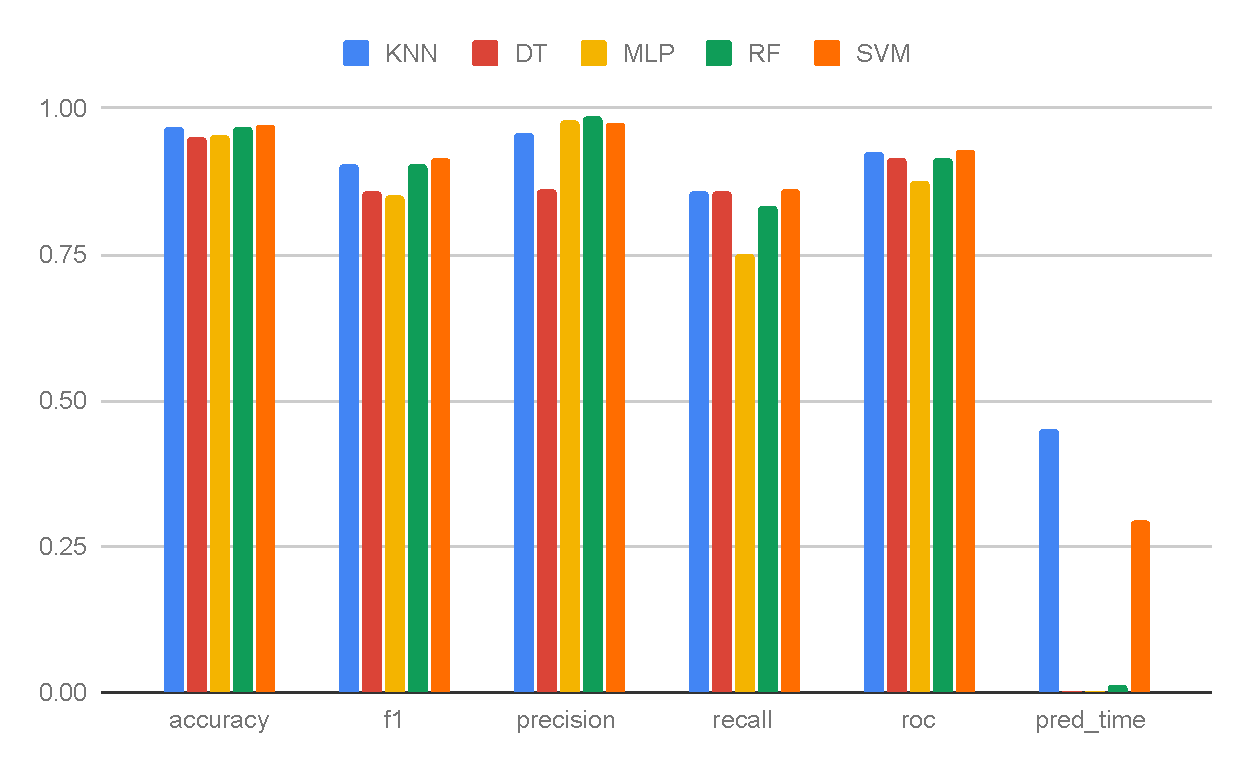
\includegraphics[width=0.9\columnwidth]{media/results/perf_ds_4.pdf}
    \caption{Performance Results Dataset 4} \label{fig:perfromance_results_dataset_4}
\end{figure}

\subsection{Performance Error Calculation}
For error calculation, best models are tested against training datasets of other models. Figure \ref{fig:perfromance_delta_knn}-\ref{fig:perfromance_delta_svm} shows the average error introduced when models are tested against training datasets of other models. This chart shows that KNN, MLP, and SVM models introduced minimum errors, whereas DT and RF models introduced large amounts of error. Figure \ref{fig:perfromance_delta_svm} also shows that SVM model produced similar error across all datasets. This smaller difference in error suggests that the SVM classifier can be used for classification tasks of similar nature.

% Decision Tree Cross-Performance
\begin{table}[hbt]
\caption{Performance of Decision Tree model trained on dataset 1}\label{tab:performance_of_decision_tree_model_trained_on_dataset_1}
\begin{tabular*}{\tblwidth}{@{}LLLLL@{}}
\toprule
    Metric & Dataset 1 & Dataset 2 & Dataset 3 & Dataset 4 \\
\midrule
    Accuracy & 0.98 & 0.94 & 0.94 & 0.94 \\
    F1 & 0.96 & 0.85 & 0.85 & 0.84 \\
    Precision & 0.95 & 0.83 & 0.84 & 0.83 \\
    Recall & 0.96 & 0.86 & 0.85 & 0.85 \\
    ROC & 0.97 & 0.91 & 0.91 & 0.90 \\
\bottomrule
\end{tabular*}
\end{table}

\begin{table}[hbt]
\caption{Performance of Decision Tree model trained on dataset 2}\label{tab:performance_of_decision_tree_model_trained_on_dataset_2}
\begin{tabular*}{\tblwidth}{@{}LLLLL@{}}
\toprule
    Metric & Dataset 1 & Dataset 2 & Dataset 3 & Dataset 4 \\
\midrule
    Accuracy & 0.94 & 0.98 & 0.94 & 0.94 \\
    F1 & 0.84 & 0.96 & 0.84 & 0.85 \\
    Precision & 0.85 & 0.96 & 0.85 & 0.85 \\
    Recall & 0.82 & 0.96 & 0.84 & 0.84 \\
    ROC & 0.89 & 0.97 & 0.90 & 0.90 \\
\bottomrule
\end{tabular*}
\end{table}

\begin{table}[hbt]
\caption{Performance of Decision Tree model trained on dataset 3}\label{tab:performance_of_decision_tree_model_trained_on_dataset_3}
\begin{tabular*}{\tblwidth}{@{}LLLLL@{}}
\toprule
    Metric & Dataset 1 & Dataset 2 & Dataset 3 & Dataset 4 \\
\midrule
    Accuracy & 0.94 & 0.94 & 0.98 & 0.94 \\
    F1 & 0.84 & 0.84 & 0.96 & 0.83 \\
    Precision & 0.84 & 0.83 & 0.95 & 0.83 \\
    Recall & 0.84 & 0.85 & 0.96 & 0.84 \\
    ROC & 0.90 & 0.90 & 0.97 & 0.90 \\
\bottomrule
\end{tabular*}
\end{table}

\begin{table}[hbt]
\caption{Performance of Decision Tree model trained on dataset 4}\label{tab:performance_of_decision_tree_model_trained_on_dataset_4}
\begin{tabular*}{\tblwidth}{@{}LLLLL@{}}
\toprule
    Metric & Dataset 1 & Dataset 2 & Dataset 3 & Dataset 4 \\
\midrule
    Accuracy & 0.94 & 0.94 & 0.95 & 0.98 \\
    F1 & 0.85 & 0.85 & 0.85 & 0.96 \\
    Precision & 0.85 & 0.85 & 0.85 & 0.96 \\
    Recall & 0.85 & 0.84 & 0.85 & 0.96 \\
    ROC & 0.91 & 0.90 & 0.91 & 0.97 \\
\bottomrule
\end{tabular*}
\end{table}

% KNN Cross-Performance
\begin{table}[hbt]
\caption{Performance of KNN model trained on dataset 1}\label{tab:performance_of_knn_model_trained_on_dataset_1}
\begin{tabular*}{\tblwidth}{@{}LLLLL@{}}
\toprule
    Metric & Dataset 1 & Dataset 2 & Dataset 3 & Dataset 4 \\
\midrule
    Accuracy & 0.97 & 0.97 & 0.97 & 0.96 \\
    F1 & 0.93 & 0.91 & 0.90 & 0.90 \\
    Precision & 0.96 & 0.95 & 0.94 & 0.94 \\
    Recall & 0.90 & 0.87 & 0.87 & 0.87 \\
    ROC & 0.94 & 0.93 & 0.93 & 0.93 \\
\bottomrule
\end{tabular*}
\end{table}

\begin{table}[hbt]
\caption{Performance of KNN model trained on dataset 2}\label{tab:performance_of_knn_model_trained_on_dataset_2}
\begin{tabular*}{\tblwidth}{@{}LLLLL@{}}
\toprule
    Metric & Dataset 1 & Dataset 2 & Dataset 3 & Dataset 4 \\
\midrule
    Accuracy & 0.96 & 0.97 & 0.96 & 0.96 \\
    F1 & 0.90 & 0.93 & 0.90 & 0.89 \\
    Precision & 0.94 & 0.96 & 0.94 & 0.94 \\
    Recall & 0.86 & 0.90 & 0.86 & 0.85 \\
    ROC & 0.92 & 0.94 & 0.92 & 0.92 \\
\bottomrule
\end{tabular*}
\end{table}

\begin{table}[hbt]
\caption{Performance of KNN model trained on dataset 3}\label{tab:performance_of_knn_model_trained_on_dataset_3}
\begin{tabular*}{\tblwidth}{@{}LLLLL@{}}
\toprule
    Metric & Dataset 1 & Dataset 2 & Dataset 3 & Dataset 4 \\
\midrule
    Accuracy & 0.96 & 0.96 & 0.97 & 0.96 \\
    F1 & 0.90 & 0.90 & 0.93 & 0.90 \\
    Precision & 0.95 & 0.95 & 0.96 & 0.94 \\
    Recall & 0.86 & 0.86 & 0.89 & 0.86 \\
    ROC & 0.92 & 0.92 & 0.94 & 0.92 \\
\bottomrule
\end{tabular*}
\end{table}

\begin{table}[hbt]
\caption{Performance of KNN model trained on dataset 4}\label{tab:performance_of_knn_model_trained_on_dataset_4}
\begin{tabular*}{\tblwidth}{@{}LLLLL@{}}
\toprule
    Metric & Dataset 1 & Dataset 2 & Dataset 3 & Dataset 4 \\
\midrule
    Accuracy & 0.96 & 0.96 & 0.96 & 0.97 \\
    F1 & 0.90 & 0.90 & 0.90 & 0.92 \\
    Precision & 0.94 & 0.95 & 0.94 & 0.96 \\
    Recall & 0.86 & 0.86 & 0.87 & 0.89 \\
    ROC & 0.92 & 0.92 & 0.93 & 0.94 \\
\bottomrule
\end{tabular*}
\end{table}

% MLP Cross-Performance
\begin{table}[hbt]
\caption{Performance of MLP model trained on dataset 1}\label{tab:performance_of_mlp_model_trained_on_dataset_1}
\begin{tabular*}{\tblwidth}{@{}LLLLL@{}}
\toprule
    Metric & Dataset 1 & Dataset 2 & Dataset 3 & Dataset 4 \\
\midrule
    Accuracy & 0.97 & 0.96 & 0.96 & 0.96 \\
    F1 & 0.92 & 0.89 & 0.89 & 0.89 \\
    Precision & 0.97 & 0.95 & 0.94 & 0.95 \\
    Recall & 0.88 & 0.85 & 0.85 & 0.85 \\
    ROC & 0.93 & 0.92 & 0.92 & 0.92 \\
\bottomrule
\end{tabular*}
\end{table}

\begin{table}[hbt]
\caption{Performance of MLP model trained on dataset 2}\label{tab:performance_of_mlp_model_trained_on_dataset_2}
\begin{tabular*}{\tblwidth}{@{}LLLLL@{}}
\toprule
    Metric & Dataset 1 & Dataset 2 & Dataset 3 & Dataset 4 \\
\midrule
    Accuracy & 0.96 & 0.97 & 0.96 & 0.96 \\
    F1 & 0.90 & 0.91 & 0.90 & 0.90 \\
    Precision & 0.95 & 0.97 & 0.94 & 0.95 \\
    Recall & 0.85 & 0.87 & 0.85 & 0.85 \\
    ROC & 0.92 & 0.93 & 0.92 & 0.92 \\
\bottomrule
\end{tabular*}
\end{table}

\begin{table}[hbt]
\caption{Performance of MLP model trained on dataset 3}\label{tab:performance_of_mlp_model_trained_on_dataset_3}
\begin{tabular*}{\tblwidth}{@{}LLLLL@{}}
\toprule
    Metric & Dataset 1 & Dataset 2 & Dataset 3 & Dataset 4 \\
\midrule
    Accuracy & 0.96 & 0.96 & 0.96 & 0.96 \\
    F1 & 0.89 & 0.89 & 0.90 & 0.88 \\
    Precision & 0.89 & 0.89 & 0.90 & 0.89 \\
    Recall & 0.88 & 0.88 & 0.91 & 0.88 \\
    ROC & 0.93 & 0.93 & 0.94 & 0.93 \\
\bottomrule
\end{tabular*}
\end{table}

\begin{table}[hbt]
\caption{Performance of MLP model trained on dataset 4}\label{tab:performance_of_mlp_model_trained_on_dataset_4}
\begin{tabular*}{\tblwidth}{@{}LLLLL@{}}
\toprule
    Metric & Dataset 1 & Dataset 2 & Dataset 3 & Dataset 4 \\
\midrule
    Accuracy & 0.95 & 0.95 & 0.95 & 0.95 \\
    F1 & 0.85 & 0.85 & 0.85 & 0.86 \\
    Precision & 0.97 & 0.97 & 0.97 & 0.98 \\
    Recall & 0.75 & 0.75 & 0.75 & 0.76 \\
    ROC & 0.87 & 0.87 & 0.87 & 0.88 \\
\bottomrule
\end{tabular*}
\end{table}

% RF Cross-Performance
\begin{table}[hbt]
\caption{Performance of RF model trained on dataset 1}\label{tab:performance_of_rf_model_trained_on_dataset_1}
\begin{tabular*}{\tblwidth}{@{}LLLLL@{}}
\toprule
    Metric & Dataset 1 & Dataset 2 & Dataset 3 & Dataset 4 \\
\midrule
    Accuracy & 0.99 & 0.97 & 0.97 & 0.97 \\
    F1 & 0.98 & 0.91 & 0.91 & 0.91 \\
    Precision & 0.99 & 0.98 & 0.97 & 0.98 \\
    Recall & 0.96 & 0.85 & 0.85 & 0.85 \\
    ROC & 0.98 & 0.92 & 0.92 & 0.92 \\
\bottomrule
\end{tabular*}
\end{table}

\begin{table}[hbt]
\caption{Performance of RF model trained on dataset 2}\label{tab:performance_of_rf_model_trained_on_dataset_2}
\begin{tabular*}{\tblwidth}{@{}LLLLL@{}}
\toprule
    Metric & Dataset 1 & Dataset 2 & Dataset 3 & Dataset 4 \\
\midrule
    Accuracy & 0.96 & 0.99 & 0.97 & 0.97 \\
    F1 & 0.90 & 0.97 & 0.91 & 0.90 \\
    Precision & 0.98 & 0.99 & 0.97 & 0.98 \\
    Recall & 0.83 & 0.96 & 0.85 & 0.84 \\
    ROC & 0.91 & 0.98 & 0.92 & 0.91 \\
\bottomrule
\end{tabular*}
\end{table}

\begin{table}[hbt]
\caption{Performance of RF model trained on dataset 3}\label{tab:performance_of_rf_model_trained_on_dataset_3}
\begin{tabular*}{\tblwidth}{@{}LLLLL@{}}
\toprule
    Metric & Dataset 1 & Dataset 2 & Dataset 3 & Dataset 4 \\
\midrule
    Accuracy & 0.96 & 0.97 & 0.99 & 0.97 \\
    F1 & 0.90 & 0.90 & 0.97 & 0.90 \\
    Precision & 0.98 & 0.98 & 0.99 & 0.98 \\
    Recall & 0.83 & 0.84 & 0.96 & 0.83 \\
    ROC & 0.91 & 0.91 & 0.98 & 0.91 \\
\bottomrule
\end{tabular*}
\end{table}

\begin{table}[hbt]
\caption{Performance of RF model trained on dataset 4}\label{tab:performance_of_rf_model_trained_on_dataset_4}
\begin{tabular*}{\tblwidth}{@{}LLLLL@{}}
\toprule
    Metric & Dataset 1 & Dataset 2 & Dataset 3 & Dataset 4 \\
\midrule
    Accuracy & 0.96 & 0.97 & 0.97 & 0.99 \\
    F1 & 0.90 & 0.91 & 0.90 & 0.97 \\
    Precision & 0.98 & 0.98 & 0.97 & 0.99 \\
    Recall & 0.84 & 0.84 & 0.85 & 0.95 \\
    ROC & 0.91 & 0.92 & 0.92 & 0.97 \\
\bottomrule
\end{tabular*}
\end{table}

% SVM Cross-Performance
\begin{table}[hbt]
\caption{Performance of SVM model trained on dataset 1}\label{tab:performance_of_svm_model_trained_on_dataset_1}
\begin{tabular*}{\tblwidth}{@{}LLLLL@{}}
\toprule
    Metric & Dataset 1 & Dataset 2 & Dataset 3 & Dataset 4 \\
\midrule
    Accuracy & 0.97 & 0.97 & 0.97 & 0.97 \\
    F1 & 0.93 & 0.92 & 0.91 & 0.91 \\
    Precision & 0.98 & 0.97 & 0.96 & 0.96 \\
    Recall & 0.89 & 0.87 & 0.87 & 0.87 \\
    ROC & 0.94 & 0.93 & 0.93 & 0.93 \\
\bottomrule
\end{tabular*}
\end{table}

\begin{table}[hbt]
\caption{Performance of SVM model trained on dataset 2}\label{tab:performance_of_svm_model_trained_on_dataset_2}
\begin{tabular*}{\tblwidth}{@{}LLLLL@{}}
\toprule
    Metric & Dataset 1 & Dataset 2 & Dataset 3 & Dataset 4 \\
\midrule
    Accuracy & 0.97 & 0.98 & 0.97 & 0.97 \\
    F1 & 0.91 & 0.94 & 0.91 & 0.91 \\
    Precision & 0.97 & 0.98 & 0.96 & 0.96 \\
    Recall & 0.86 & 0.89 & 0.86 & 0.86 \\
    ROC & 0.92 & 0.94 & 0.93 & 0.92 \\
\bottomrule
\end{tabular*}
\end{table}

\begin{table}[hbt]
\caption{Performance of SVM model trained on dataset 3}\label{tab:performance_of_svm_model_trained_on_dataset_3}
\begin{tabular*}{\tblwidth}{@{}LLLLL@{}}
\toprule
    Metric & Dataset 1 & Dataset 2 & Dataset 3 & Dataset 4 \\
\midrule
    Accuracy & 0.97 & 0.97 & 0.98 & 0.97 \\
    F1 & 0.91 & 0.92 & 0.94 & 0.91 \\
    Precision & 0.97 & 0.97 & 0.98 & 0.97 \\
    Recall & 0.85 & 0.87 & 0.89 & 0.87 \\
    ROC & 0.92 & 0.93 & 0.94 & 0.93 \\
\bottomrule
\end{tabular*}
\end{table}

\begin{table}[hbt]
\caption{Performance of SVM model trained on dataset 4}\label{tab:performance_of_svm_model_trained_on_dataset_4}
\begin{tabular*}{\tblwidth}{@{}LLLLL@{}}
\toprule
    Metric & Dataset 1 & Dataset 2 & Dataset 3 & Dataset 4 \\
\midrule
    Accuracy & 0.97 & 0.97 & 0.97 & 0.97 \\
    F1 & 0.91 & 0.91 & 0.91 & 0.93 \\
    Precision & 0.97 & 0.96 & 0.96 & 0.98 \\
    Recall & 0.85 & 0.86 & 0.86 & 0.88 \\
    ROC & 0.92 & 0.93 & 0.93 & 0.94 \\
\bottomrule
\end{tabular*}
\end{table}

\begin{figure}[btp]
    \centering
    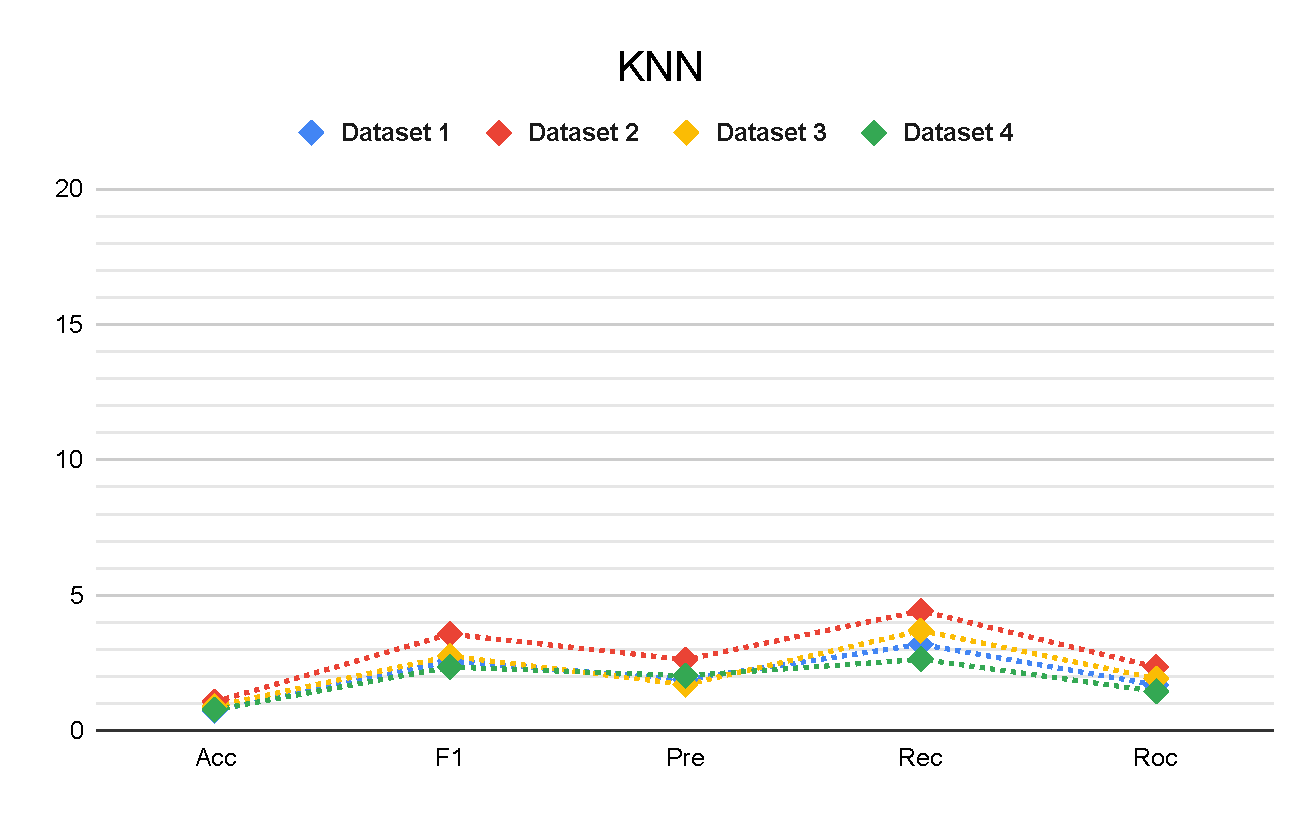
\includegraphics[width=0.9\columnwidth]{media/results/delta_KNN.pdf}
    \caption{Average Error for KNN model} \label{fig:perfromance_delta_knn}
\end{figure}

\begin{figure}[btp]
    \centering
    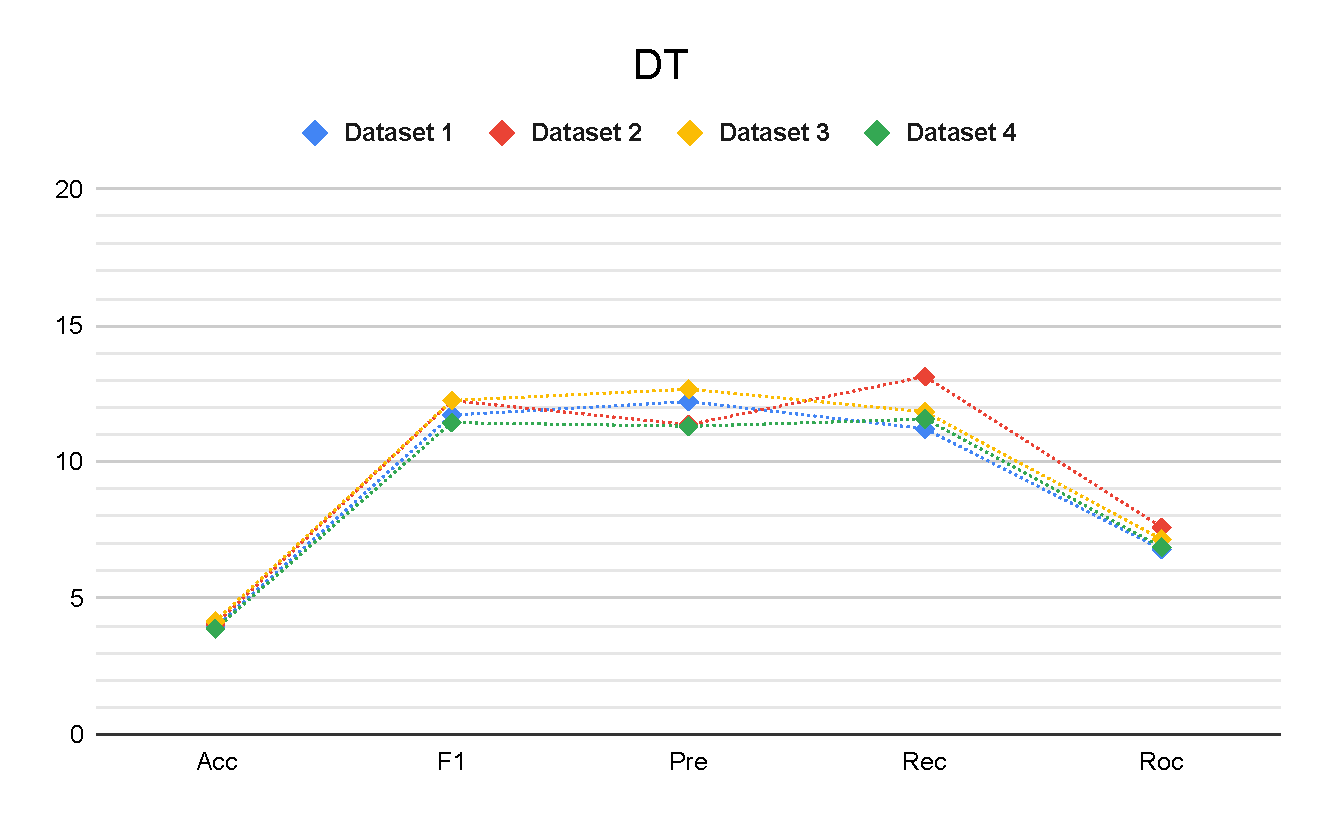
\includegraphics[width=0.9\columnwidth]{media/results/delta_DT.pdf}
    \caption{Average Error for DT model} \label{fig:perfromance_delta_dt}
\end{figure}

\begin{figure}[btp]
    \centering
    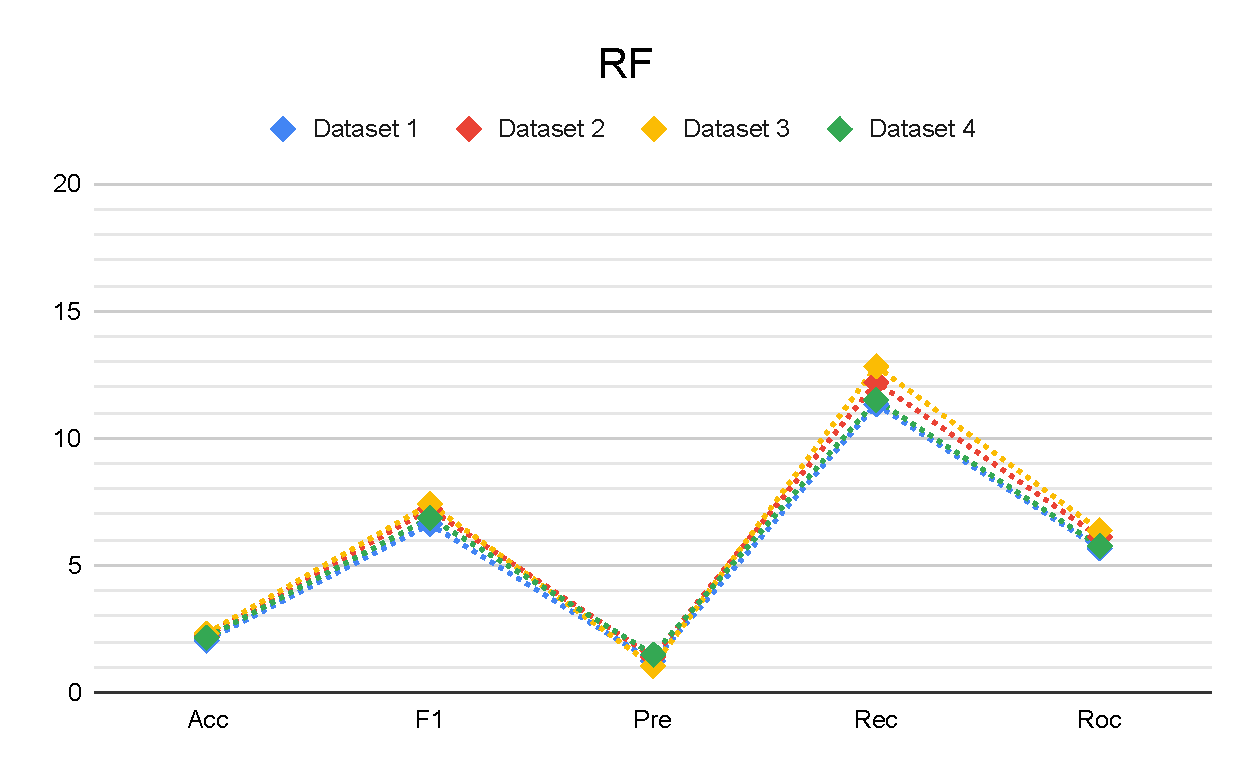
\includegraphics[width=0.9\columnwidth]{media/results/delta_RF.pdf}
    \caption{Average Error for RF model} \label{fig:perfromance_delta_rf}
\end{figure}

\begin{figure}[btp]
    \centering
    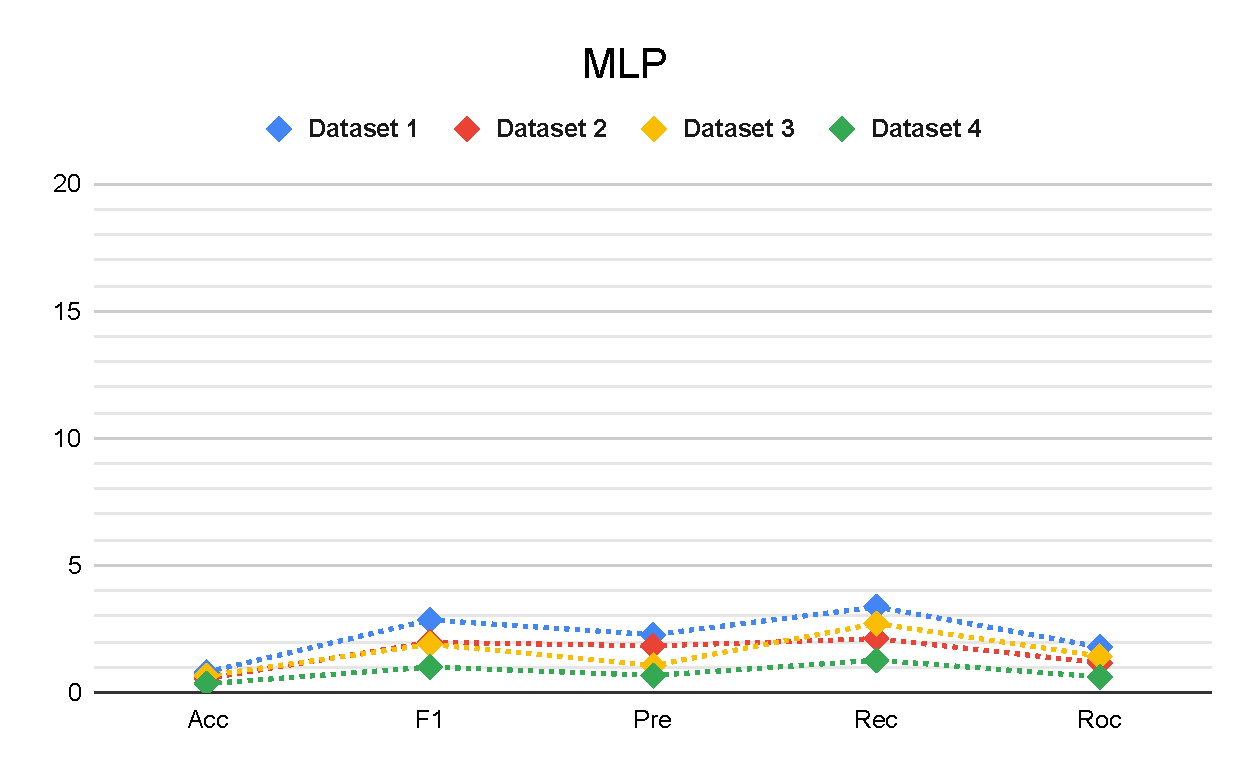
\includegraphics[width=0.9\columnwidth]{media/results/delta_MLP.pdf}
    \caption{Average Error for MLP model} \label{fig:perfromance_delta_mlp}
\end{figure}

\begin{figure}[!tb]
    \centering
    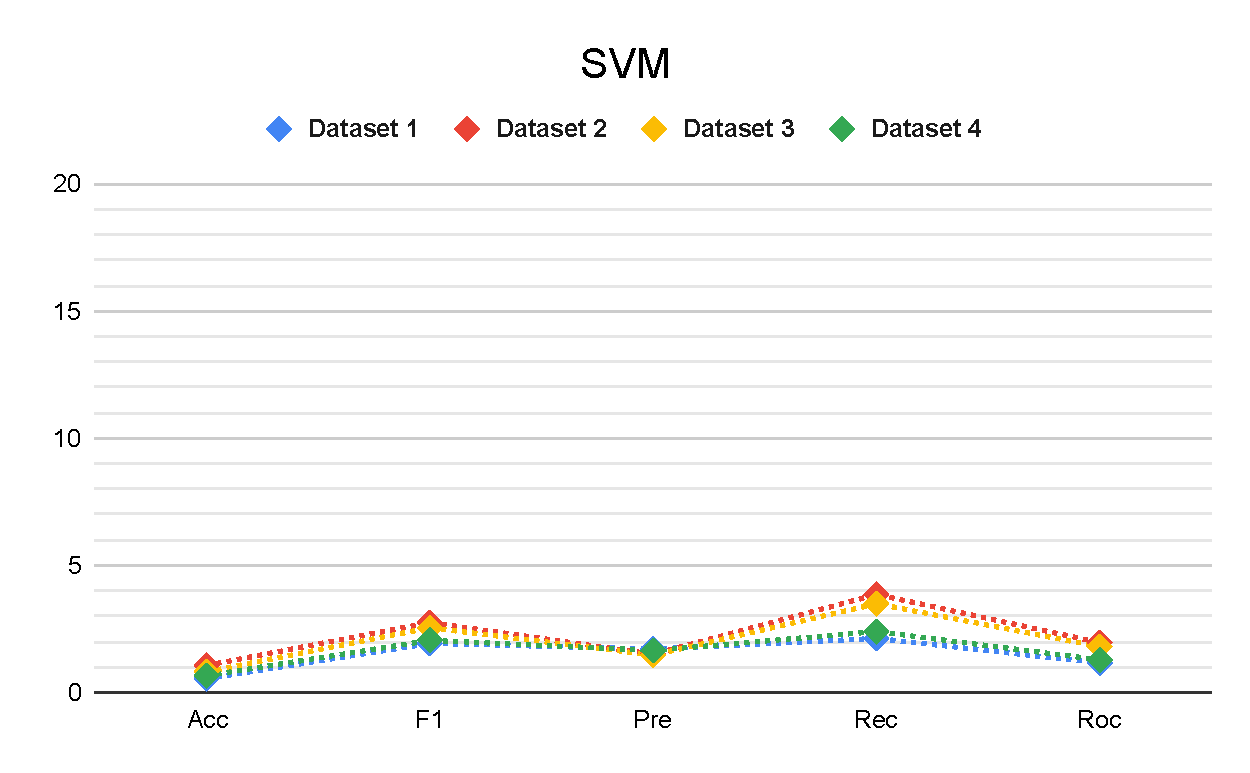
\includegraphics[width=0.9\columnwidth]{media/results/delta_SVM.pdf}
    \caption{Average Error for SVM model} \label{fig:perfromance_delta_svm}
\end{figure}
